\documentclass[assd_tp3_main.tex]{subfiles}

\begin{document}

\section{SAR}

\subsection{Introducci\'on}

El primer conversor que se implement\'o fue un registro de aproximaciones sucesivas, o SAR por sus siglas en ingl\'es (Successive Approximation Register). El diagrama de bloques de este conversor se observa en la figura \ref{fig:sar-bloques}.


\begin{figure}[ht!]
	\centering
	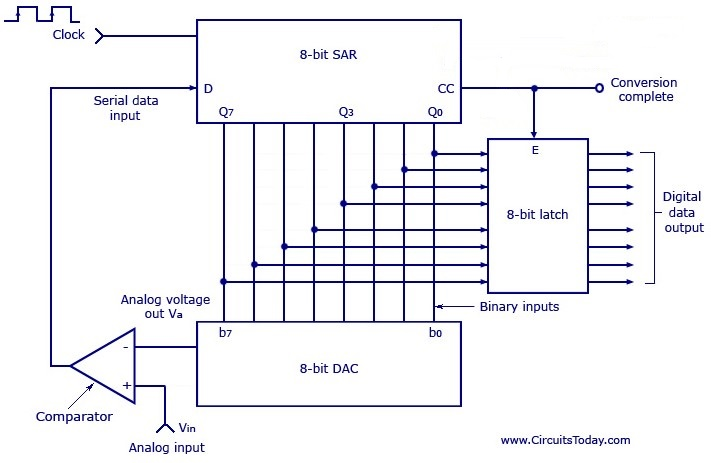
\includegraphics[width=0.8\textwidth]{images/ej2/sar-bloques.jpg}
	\caption{Diagrama en bloques del SAR}
	\label{fig:sar-bloques}
\end{figure}

La l\'ogica de predicci\'on del SAR sigue el principio de la b\'usqueda binaria. Se comienza con el bit m\'as significativo en 1 y el resto en 0, se convierte esta se\~nal al dominio anal\'ogico, y se la compara con la entrada. Seg\'un el resultado de esta comparaci\'on (a la cual se la puede considerar una cuantizaci\'on de un bit), el bit se dejar\'a encendido o se apagar\'a en la siguiente iteraci\'on, en la cual adem\'as se encender\'a el bit siguiente. El proceso se repite sucesivamente hasta llegar al bit menos significativo, luego de lo cual se enciende la se\~nal de end of conversion, guardando el resultado de la conversi\'on en el latch de salida. Como para cada conversi\'on de N bits se deben hacer N comparaciones, y un pulso adicional para obtener la nueva muestra,  entonces se requiere que la frecuencia del clock que controla al registro de aproximaciones sucesivas sea:

\begin{equation}
	f_{CLK} = 9f_s
\end{equation} 

Adicionalmente, es necesario que la se\~nal de entrada se mantenga constante durante el tiempo de conversi\'on, o al menos que var\'ie menos de un LSB. por lo tanto, la misma debe atravesar un sample and hold antes de ingresar al comparador.



\subsection{Implementaci\'on}

Para la implementaci\'on, se utiliz\'o un sample and hold LF398, un comparador LM311 y un DAC0800 con un LM398 como amplificador de transimpedancia, tal como se explic\'o para la placa base ADA. Tanto el registro de aproximaciones sucesivas como el latch se implementaron con la FPGA, que a su vez controlaba el input l\'ogico del sample and hold. 


\subsection{Mediciones}

La precisi\'on del conversor se vio confirmada por las mediciones realizadas en continua, tal como se observa en la figura \ref{fig:sar-continua}.

\begin{figure}[htb!]
	\centering
	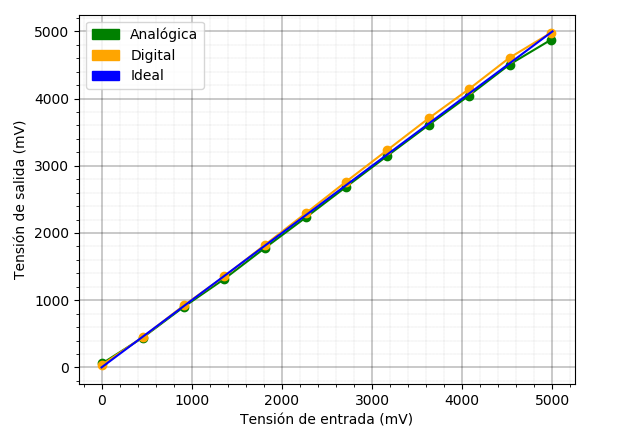
\includegraphics[width=\textwidth]
	{images/ej2/sar-continua.png}
	\caption{Salida del SAR con entrada continua}
	\label{fig:sar-continua}
\end{figure}

Un problema que se observa en continua es que cuando la entrada es de 5V, la tensi\'on de full scale, no se obtienen 5V a la salida. Efectivamente, en la figura \ref{fig:sar-fs} se puede confirmar que el conversor presenta problemas para llegar a los extremos del rango donde deber\'ia funcionar. Esto puede deberse a inexactitud en las resistencias usadas en el conversor digital-anal\'ogico, lo cual ser\'ia consistente con el hecho de que el error es mayor en la salida anal\'ogica que en la digital.

\begin{figure}
	\centering
	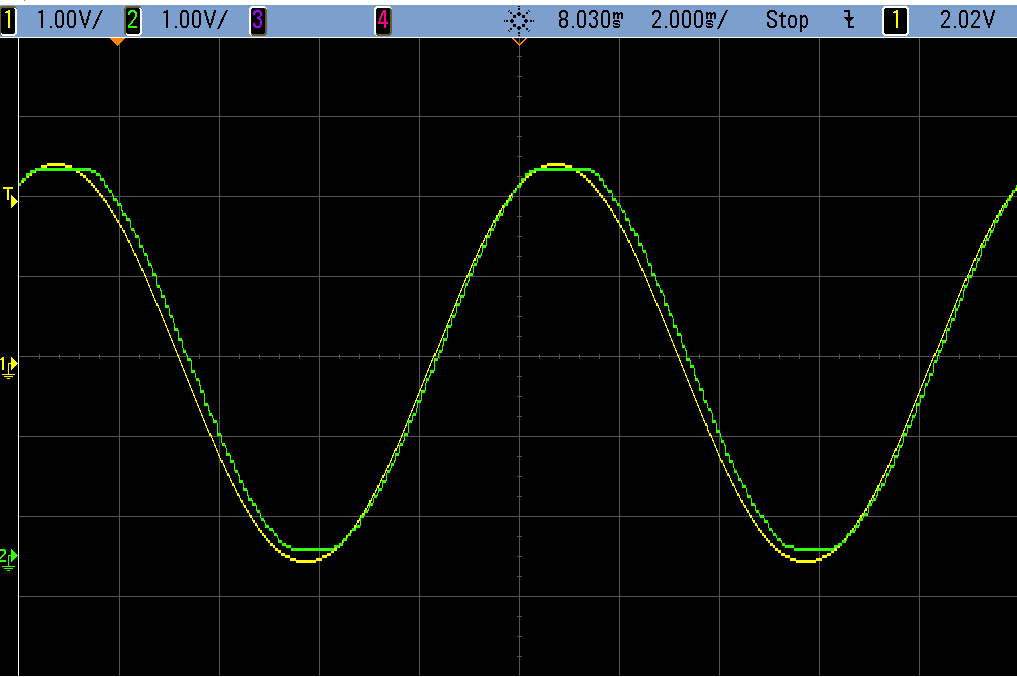
\includegraphics[width=0.7\textwidth]
	{images/ej2/ss_.png}
	\caption{Salida del SAR con entrada de 5V pico a pico}
	\label{fig:sar-fs}
\end{figure}

\begin{figure}[htb!]
	\centering
	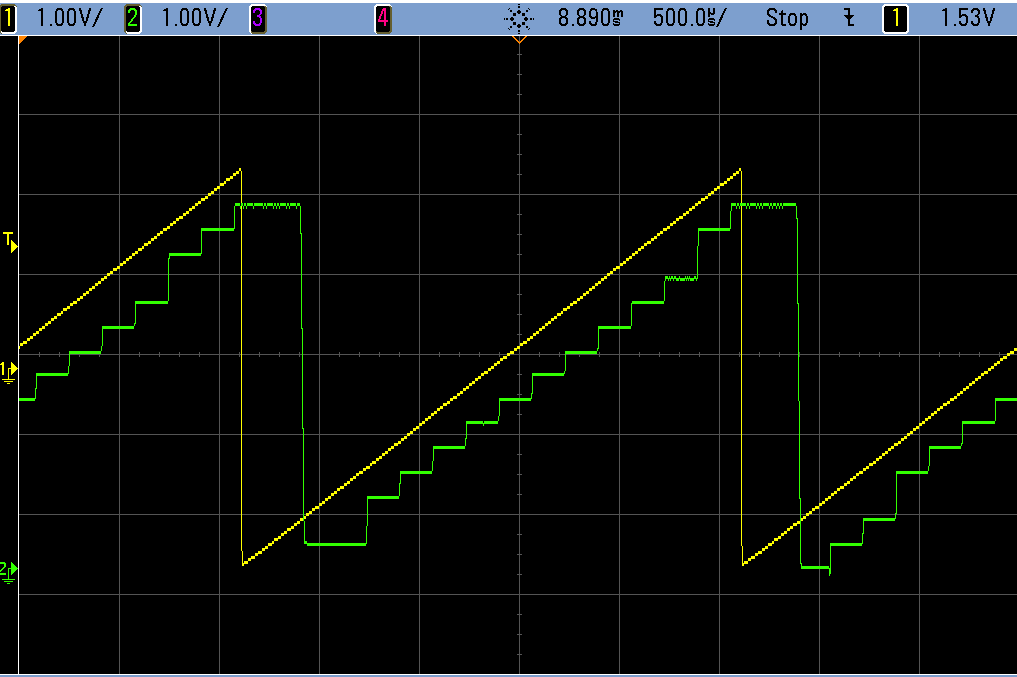
\includegraphics[width=0.45\textwidth]
	{images/ej2/s_4.png}
	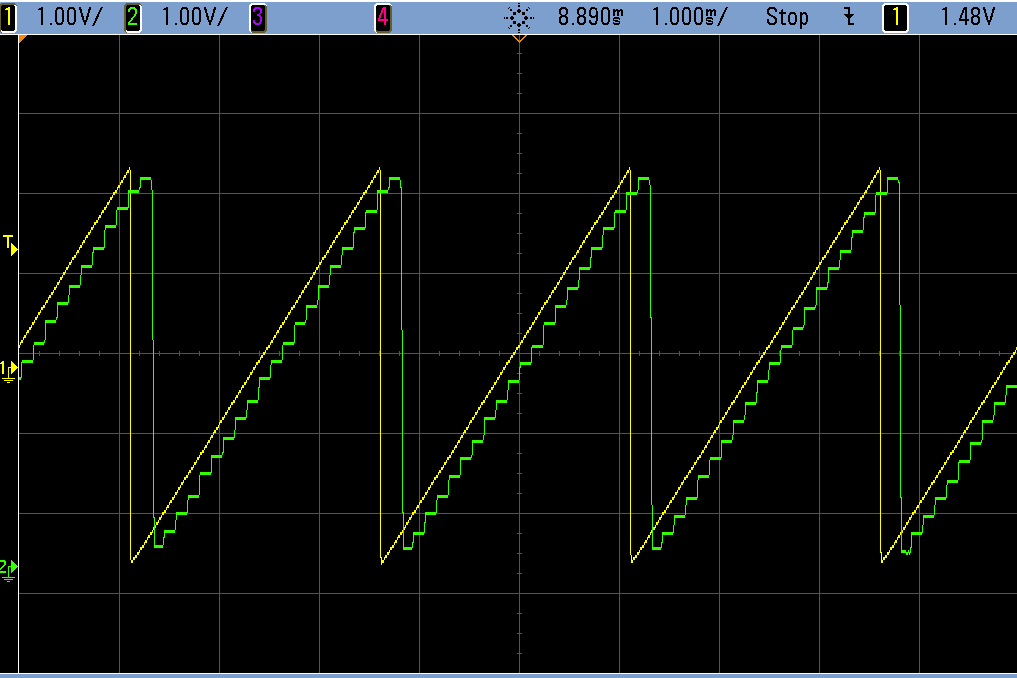
\includegraphics[width=0.45\textwidth]
	{images/ej2/s_8.png}
	\caption{Salida del SAR con 4 y 6 bits activos}
	\label{fig:sar-bits}
\end{figure}

Se estudi\'o, asimismo, el efecto de reducir la cantidad de bits activos. Esto podr\'ia, en teor\'ia, resultar en una frecuencia de clock menor, pero esto no se implement\'o en la FPGA, con lo cual la frecuencia de muestreo se mantiene constante. Se observa que aparece una mayor cantidad de niveles discretos. con mayor cantidad de bits encendidos.

\begin{figure}[htb!]
	\centering
	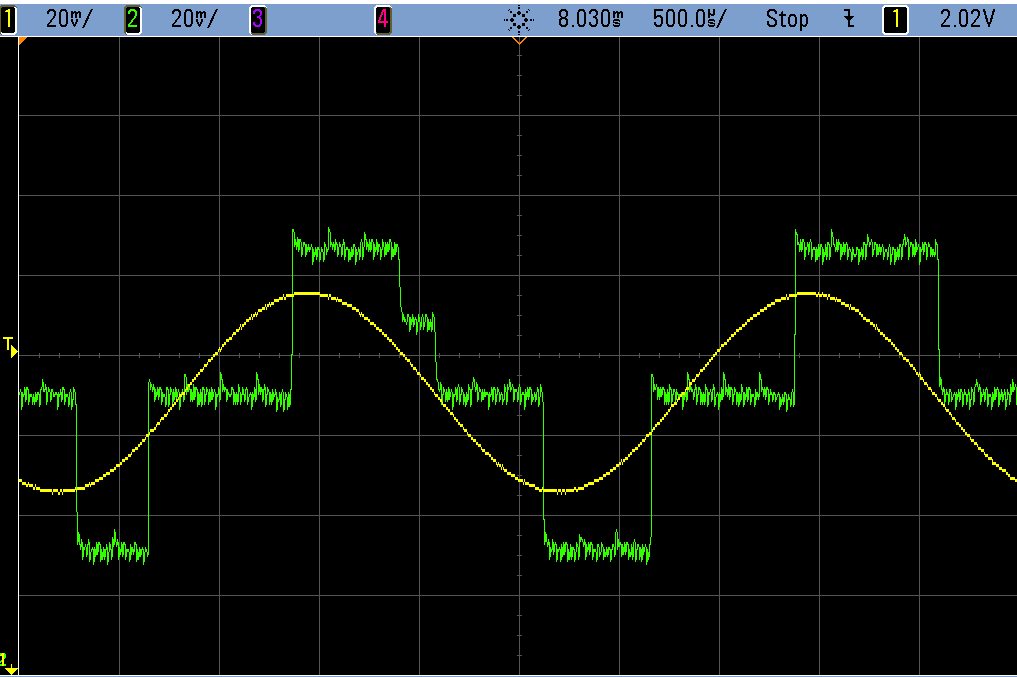
\includegraphics[width=\textwidth]
	{images/ej2/s__.png}
	\caption{Salida del SAR con entrada de 25mV de amplitud}
	\label{fig:sar-chiquita}
\end{figure}

El comportamiento del sistema con una se\~nal de 25mV de amplitud se puede ver en la figura \ref{fig:sar-chiquita}. Aqu\'i el error que se observa en la entrada y la salida es significativo, lo cual sugerir\'ia una pobre inmunidad al ruido del sistema.


\end{document}

